\chapter{Informatisation des infrastructures}

L'idée des smart cities et de l'informatisation de la gestion des villes n'est pas nouvelle.
Il y a eu beaucoup d'idée du type science fiction dans les années 1800 qui pensais la ville
complètement automatisé par des tubes, des trottoir roulant, une gestion des déchets automatique.
Cette science fiction à mis presque 150ans à voir le jours.

\begin{figure}[h]
  \centering
  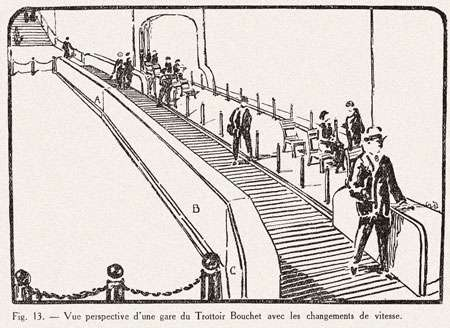
\includegraphics[scale=0.30]{media/trottoir_roulant.jpg}
  \caption{Trottoir roulant - Paris 1900 - Exposition Universelle}
\end{figure}

\section{Étude de Cybersyn}

Dans les années 1970 au Chili, Salvador Allende gagne les élections présidentielles.
En pleine guerre froide, le Chili devenu Socialiste se déclare neutre et n'est donc
contraint ni par les États Unis, ni par l'URSS.

Le Chili a vu dans les années précédentes d'importantes famines, le gouvernement voulais
absolument éviter ça, malheureusement, vu que le gouvernement est socialiste, tout passe
par un rationnement et toutes les décisions sont pris d'en haut.
Pour éviter de finir comme l'URSS, qui a connus d'importantes famines dût a une
bureaucratie écrasante, l'état demanda à Fernando Flores de trouver une solution.

Fernando Flores, est un ingénieur, entrepreneur et politicien chilien qui eu l'idée
d'automatiser le pays, car tout ce qui permet d'aller vite évite la rétention d'information,
ainsi que des ralentissement inutile pour l'avenir du pays.
Il décida d'inviter Stafford Beer pour s'occuper d'un tout nouveau projet d'une grande ampleur,
le projet Cybernet pour Cybernetic Synergy.

L'idée de base est simple, obtenir en temps réel (c'est à dire 1 fois par jours pour l'époque)
l'état économique du pays pour faire les bonnes décisions.
Pour ce faire, chaque entité connecté au réseau devais envoyer un compte-rendu quotidien sur
la production de celle-ci, ce compte-rendu est envoyé au niveau supérieur et est mis en commun
avec les autres entité.

\begin{figure}[h!]
  \centering
  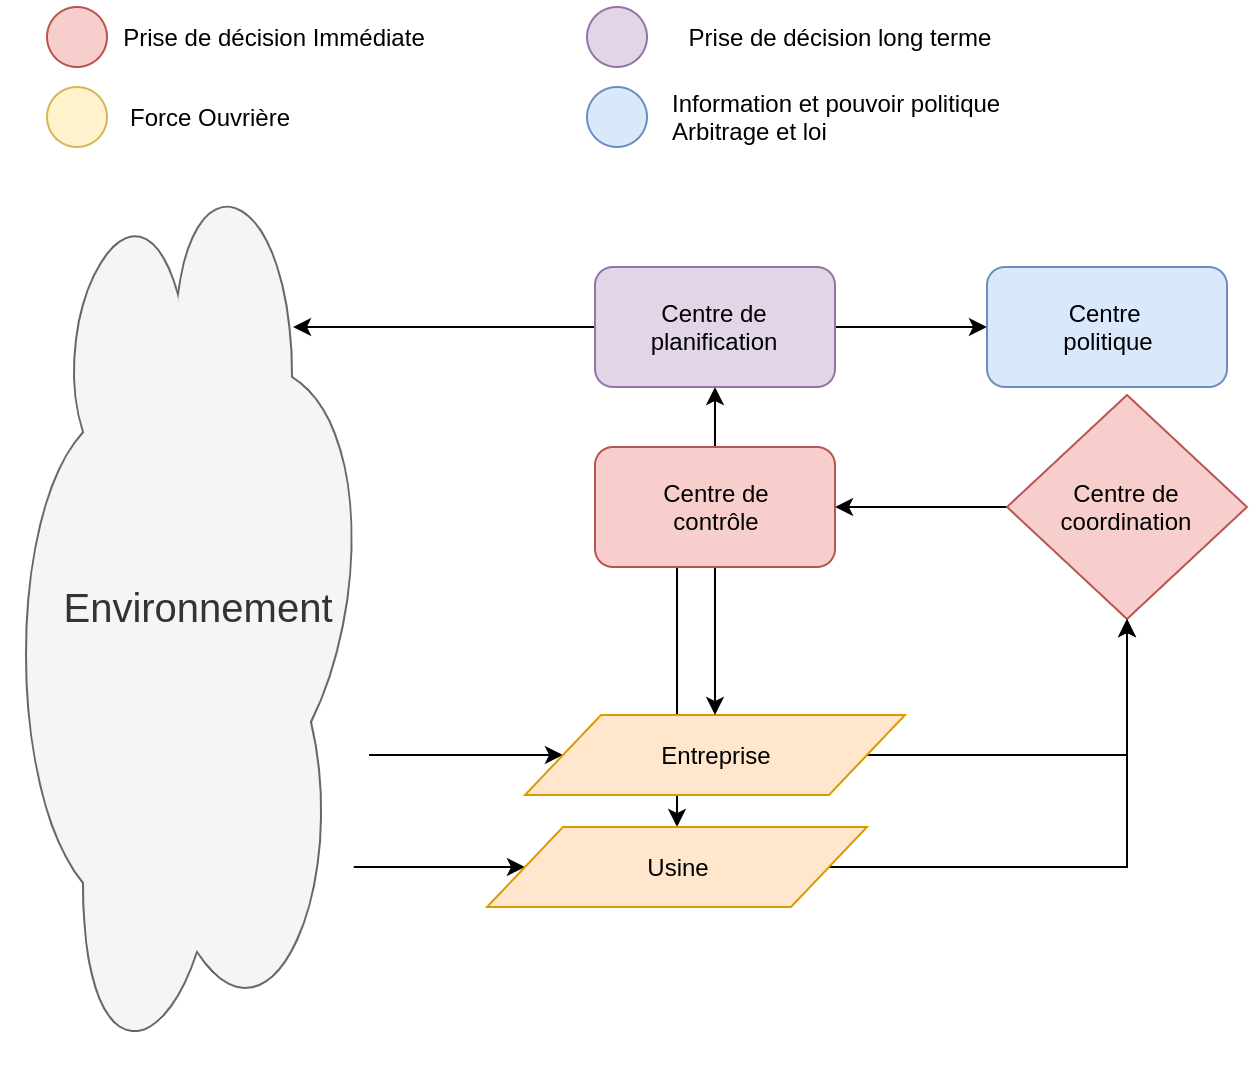
\includegraphics[scale=0.20]{media/cybersyn.png}
  \caption{Architecture du projet CyberSyn}
\end{figure}

Le projet avais de nombreux avantages, les travailleurs remontais les informations,
il y avais une notion d'intelligence artificielle qui traitais cette donnée pour en extraire
le plus important, et pour finir, le système faisait des simulations pour les jours suivant.

L'un des points les plus impréssionnant est le fait d'avoir réussi un tel projet avant
l'invention d'internet, tout passait par un système fait maison appelé Telex.
Telex fut développé avec un seul et unique ordinateur en n'en simulant plusieurs milliers.

Malheureusement le projet pris fin en 1973 en même temps que le gouvernement de Salvador Allende.
La révolution Chilienne et le poutch miliaire détruira ainsi 3ans d'un projet futuriste ayant
énormément coûté au gouvernement.

Ce qu'il faut retenir de ce projet est crucial, un investissement dans la smart grid prend du temps,
c'est coûteux et cela demande de garder en permanence des personnes comprenant bien le projet.
Le poutch militaire mis les scientifiques du projet hors du pays, par conséquent plus personne ne pouvais
le piloté.

Par la suite, Stafford Beer continua ses recherches sur la Théorie des systèmes viables.

% Il manque le sujet de la récursivité
% Ainsi que du fait que ce projet donna 1an de sursit au gouvernement avant sa fin


% 1970 Chili
% Salvador Allende au pouvoir
% Régime Socialiste / Proche Communisme
% Nationalisation
% Intervenant de l'état dans les entreprises - Incompétences + Corruption
% Fernando Flores propose une idée de Smart Grid
% Idée qui viens de Stafford Beer, un cyberneticien
% Theorie des systèmes viables

% Cybernetique : Automatisme, Intéligence artificielle, Réseaux
% Terme vieux

% Projet Cybersyn => Cybernetic Synergy

% Context : Pas encore internet - Arpanet née en 1969

% Sujet du projet : La Planification
% - L'état doit pouvoir planifier tout un pays (Régime Socialiste)
% - Donner (illusion) du pouvoir aux ouvriers

% Problèmes a résoudres :
% - Bureaucratie
% - Rétention d'information
% - Famines


% 1 - Production et information venue des travailleurs
% 2 - Prises de decision - Data analysis et IA
% 3 - Simulation long terme et planification
% 4 - Arbitrage

% Liberté = Interdependence

% Pour simplifier la mise en place - Le model était récursif
% 12 niveaux de récursion

% 12 - Nation
% 11 - Gouvernement
% 10 - Économie
% 09 - Industrie
% 08 - Branche d'industrie
% 07 - Secteur d'industrie
% 06 - Sous-domaine
% 05 - Entreprise
% 04 - Département
% 03 - Atelier
% 02 - Équipe
% 01 - Travailleur

% Autonomie du systèmes tout en faisant partit d'un tout

% Réseau telex

% Formation :
% - Formateurs
% - Dessin animé
% - Chansons

% Utilité du projet (avant sa mort) :
% - Connaitre l'état économique du pays (en quelques jours contre des mois)
% - Pouvoir prévenir les crises (grève - sabotage)

% Echec :

% Projet lancé en 1971 - Coup d'état en 1973
% 20\% des entreprises connecté au réseau

% Avant sa fin de vie, Sybersync n'intégra que le niveau 05 au niveau 09

% Projet trop complexe - peu de gens le comprenaient
% ouvriers jamais impliquer dans le processus

% Technologie trop avangardiste

% Reflexions sur le projet :

% Projet ambitieux surtout pour son époque
% Pouvant servire pour l'intéret general ou pour un dictateur en fonction de peu de critères

% La surveillance et l'information sont le nerf du fonctionnement de ce genre de systèmes

% Notes de l'interview de Eden Medina
% https://www.youtube.com/watch?v=9qKoaQo9GTw

% Il y avais 50 ordinateurs au Chili en 1971
% 4 ordinateurs de l'état
% dont 1 du projet cybersyn

% Le projet a imaginer un réseau national de plusieurs miliers d'ordinateurs
% avec 1 seul

\section{Protocoles et Open Data}
% Communication entre services différents (voiture - infrastructure - éclairage - chauffage)
% Centralisation TaaS (Pilot Things)
\section{Gestion des catastrophes}
% Panne électrique par exemple
\section{Optimisation de la distribution énergétique}
\section{Cas d'étude d'une bourse de l'energie}
